%\title{LaTeX Portrait Poster Template}
%%%%%%%%%%%%%%%%%%%%%%%%%%%%%%%%%%%%%%%%%
% a0poster Portrait Poster
% LaTeX Template
% Version 1.0 (22/06/13)
%
% The a0poster class was created by:
% Gerlinde Kettl and Matthias Weiser (tex@kettl.de)
% 
% Adapter by Jens Buysse for Hogeschool Gent
% This template has been downloaded from:
% http://www.LaTeXTemplates.com
%
% License:
% CC BY-NC-SA 3.0 (http://creativecommons.org/licenses/by-nc-sa/3.0/)
%
%%%%%%%%%%%%%%%%%%%%%%%%%%%%%%%%%%%%%%%%%

%----------------------------------------------------------------------------------------
%	PACKAGES AND OTHER DOCUMENT CONFIGURATIONS
%----------------------------------------------------------------------------------------

\documentclass[a0,portrait]{a0poster}

\usepackage{multicol} % This is so we can have multiple columns of text side-by-side
\columnsep=100pt % This is the amount of white space between the columns in the poster
\columnseprule=3pt % This is the thickness of the black line between the columns in the poster

\usepackage[svgnames]{xcolor} % Specify colors by their 'svgnames', for a full list of all colors available see here: http://www.latextemplates.com/svgnames-colors

\usepackage{times} % Use the times font
%\usepackage{palatino} % Uncomment to use the Palatino font

\usepackage{graphicx} % Required for including images
\graphicspath{{figures/}} % Location of the graphics files
\usepackage{booktabs} % Top and bottom rules for table
\usepackage[font=small,labelfont=bf]{caption} % Required for specifying captions to tables and figures
\usepackage{amsfonts, amsmath, amsthm, amssymb} % For math fonts, symbols and environments
\usepackage{wrapfig} % Allows wrapping text around tables and figures
\usepackage[export]{adjustbox}

\begin{document}

%----------------------------------------------------------------------------------------
%	POSTER HEADER 
%----------------------------------------------------------------------------------------

% The header is divided into two boxes:
% The first is 75% wide and houses the title, subtitle, names, university/organization and contact information
% The second is 25% wide and houses a logo for your university/organization or a photo of you
% The widths of these boxes can be easily edited to accommodate your content as you see fit

\begin{minipage}[t]{0.75\linewidth}
\veryHuge \color{HoGentAccent1} \textbf{Growth hacking voor een niet-technologische Brusselse start-up: zoektocht naar versnelde community-groei} \color{Black}\\ % Title
\Huge\textit{}\\[2.4cm] % Subtitle
\huge \textbf{Vanderstadt Evert, Van Meervenne Michiel, Antjon Tom}\\[0.5cm] % Author(s)
\huge Hogeschool Gent, Valentin Vaerwyckweg 1, 9000 Gent\\[0.4cm] % University/organization
\Large \texttt{evert.vanderstadt.w9991@hogent.be} \\
\end{minipage}
%
\begin{minipage}[t]{0.25\linewidth}

\includegraphics[width=13cm,right]{figures/HG-beeldmerk-woordmerk.png} 

\end{minipage}

\vspace{1cm} % A bit of extra whitespace between the header and poster content

%----------------------------------------------------------------------------------------

\begin{multicols}{2} % This is how many columns your poster will be broken into, a portrait poster is generally split into 2 columns

%----------------------------------------------------------------------------------------
%	ABSTRACT
%----------------------------------------------------------------------------------------

\color{HoGentAccent1} % Navy color for the abstract

\begin{abstract}
Growth hacking wordt vaak uitgelegd aan de hand van de grote succesverhalen van Airbnb, Spotify en andere grote techbedrijven die op korte tijd heel snel gegroeid zijn. Het toepassen van deze marketingtechniek op een niet-technologische Brusselse start-up met een fysiek product wordt in deze bachelorproef onderzocht.
\end{abstract}
%----------------------------------------------------------------------------------------
%	INTRODUCTION
%----------------------------------------------------------------------------------------

\begin{center}\vspace{1cm}
	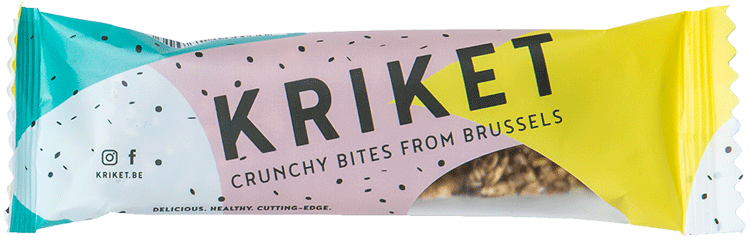
\includegraphics[width=1.0\linewidth]{kriketbar}
	\captionof{figure}{\color{HoGentAccent5} De eerste Belgische krekelreep.}
\end{center}


\color{HoGentAccent1} 
\section*{Introductie}
\color{black}
Kriket is een Brusselse start-up die krekelrepen produceert en verkoopt via lokale handelaars, partners én hun eigen webshop. 

Iedere start-up wil groeien, dit geldt ook voor Kriket, maar vaak bezitten start-ups niet over het gigantische marketingbudget van hun concurrenten. Dan ontstaat de vraag rond goedkope marketing en snelle groei; is het mogelijk?

Om deze vraag te beantwoorden wordt er eerst onderzoek gevoerd rond een interessante marketingstrategie. Het resultaat is ``growth hacking``, waar de werkvelden marketing en IT samenkomen (zie figuur~2). Het is een term die frequent gebruikt wordt, maar toch is er veel onduidelijkheid rond.

Dit is dan de eerste belangrijke vraag: onderzoeken wat growth hacking nu écht betekent. Zodra dit duidelijk is kan men het onderzoek starten naar de toepasbaarheid op Kriket, een niet-technologische Brusselse start-up met een fysiek product. 

Het is niet vanzelfsprekend dat het voor een niet-technologische start-up ook kan werken, aangezien alle voorbeelden van succesvolle growth hacks toegepast zijn op start-ups die een webplatform als product hebben. Dit zijn dus steeds online of technologische start-ups.

%----------------------------------------------------------------------------------------
%	GEOLOGY
%----------------------------------------------------------------------------------------

\color{Black} % DarkSlateGray color for the rest of the content
\color{HoGentAccent1} 
\section*{Onderzoek}
\color{black}

Het onderzoek wordt gevoerd aan de hand van interviews met experts in het werkveld. De geïnterviewden zijn gespecialiseerd in verschillende onderdelen die gebruikt worden bij growth hacking (zie figuur~2). Dit gaat van het creatieve deel in marketing tot het technisch opvangen en analyseren van alle data. 

De vragen zijn nauwkeurig opgesteld met een grondige literatuurstudie als basis. Er is bewust niet gekozen voor het afnemen van enquêtes, want interviews geven de mogelijkheid om dieper in te gaan op bepaalde onderwerpen. Zo kan de geïnterviewde onder andere meer uitleg geven over de vragen waar hij of zij gespecialiseerd in is.

\color{HoGentAccent1} 
%  \section*{Sectie met figuur}
\color{black}

\begin{center}
\vspace{1cm}

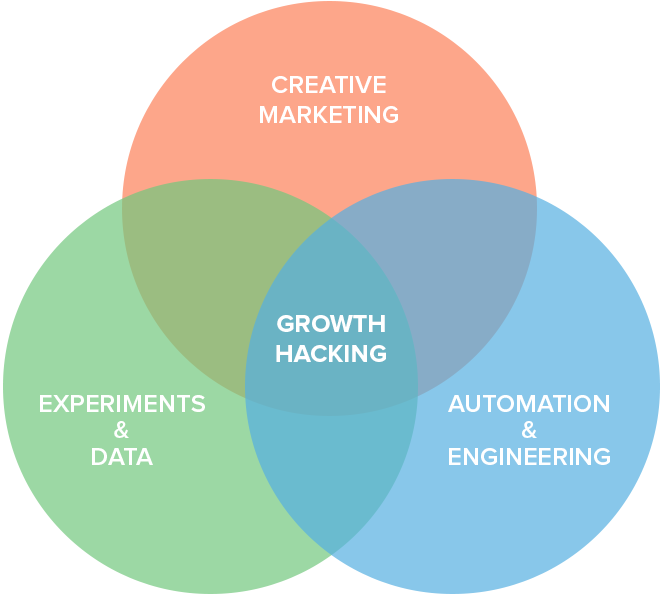
\includegraphics[width=0.9\linewidth]{growth-hacking-essential-parts}
\captionof{figure}{\color{HoGentAccent5} Essentiële onderdelen van growth hacking.}

\end{center}\vspace{1cm}

%------------------------------------------------



\color{HoGentAccent1} 
\section*{Conclusies}
\color{black}
De onderzoeksvraag waar men een antwoord op wil krijgen is de volgende:

\emph{Kan growth hacking toegepast worden op een niet-technologische Brusselse start-up met een fysiek product?}

Het eenvoudige antwoord op deze vraag is: \textbf{``Ja, het kan``}.

Dat is wat alle experts in de interviews vermelden, maar daar stopt het niet. Naast deze belangrijke conclusie zijn er voor Kriket enkele zaken om rekening mee te houden. Ook zijn er interessante ideeën naar boven gekomen bij de interviews. Eén van die ideeën is het uitwerken van een volledig digitaal platform met een abonnement-formule zoals HelloFresh en vele andere Amerikaanse voorbeelden. 

Ter verduidelijking wordt de implementatie van een growth hack op Kriket in stappen uitgeschreven. Het voorbeeld is een referral-systeem, een growth hack die bekend is door Dropbox met hun \emph{two-way} referral-systeem (zie figuur~3). Dit wordt uitgewerkt op basis van de literatuurstudie en informatie die verkregen werd tijdens de interviews. 

Naast dit voorbeeld zijn er vele ideeën die Kriket reeds toepast, zoals de samenwerkingen met grote bedrijven (zie figuur~4), influencers, enz.

\begin{center}
	\vspace{1cm}
	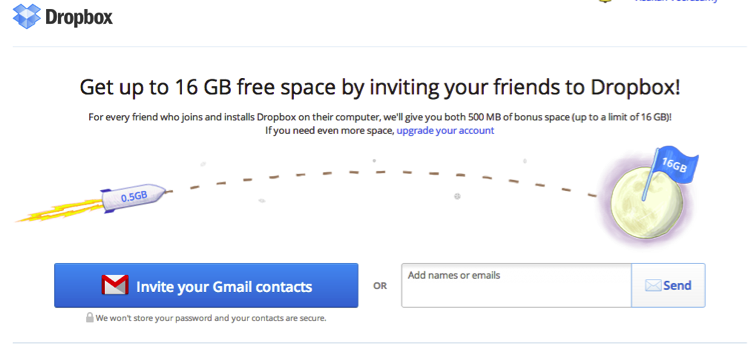
\includegraphics[width=1.0\linewidth]{dropbox-referral}
	\captionof{figure}{\color{HoGentAccent5} Het referral-systeem, de growth hack die bij Dropbox zorgde voor een groei van 3900\% in 15 maanden tijd.}
\end{center}

%----------------------------------------------------------------------------------------
%	FORTHCOMING RESEARCH
%----------------------------------------------------------------------------------------
\color{HoGentAccent1} 
\section*{Toekomstig onderzoek}
\color{black}

Wat na dit onderzoek zeker belangrijk zal zijn voor Kriket en alle andere niet-technologische start-ups is de implementatie van een (of meerdere) growth hack(s). Hier zou men onderzoek kunnen voeren rond de invloed van de growth hack op het bedrijf. De analyse kan gemaakt worden op basis van de cijfers uit Google Analytics voor de website en de verkoopcijfers. Uit deze data kan men dan vaststellen of de implementatie van de growth hack succesvol was.

\begin{center}
	\vspace{1cm}
	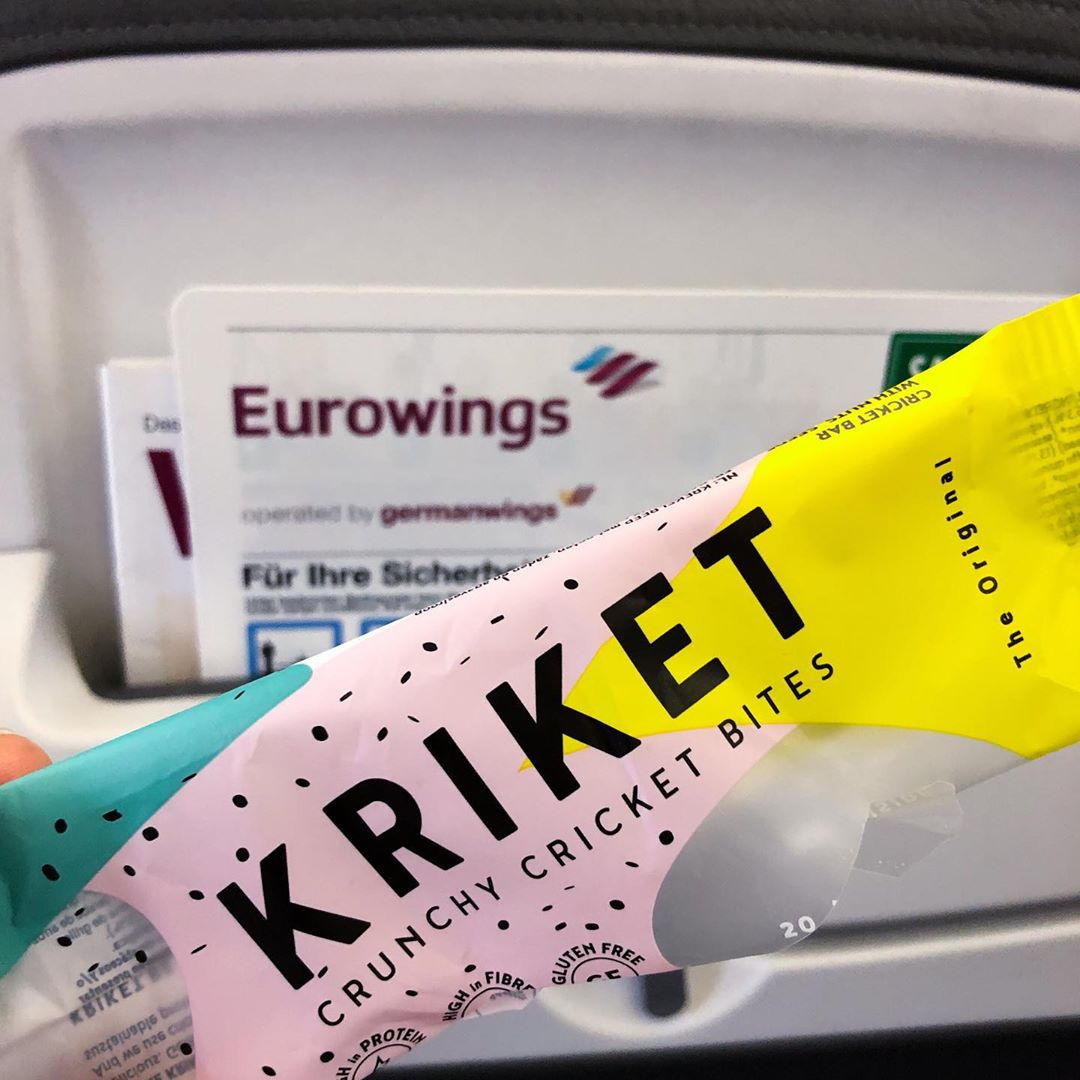
\includegraphics[width=0.9\linewidth]{kriket-eurowings}
	\captionof{figure}{\color{HoGentAccent5} Kriket breekt door! De krekelrepen zijn te vinden op je vlucht met Eurowings, in Delhaize, automaten op school, bij lokale handelaars, enz. De samenwerking met deze bedrijven zijn cruciaal voor de groei van Kriket.}
\end{center}

%----------------------------------------------------------------------------------------

\end{multicols}
\end{document}